\documentclass[tikz,border=6pt]{standalone}
\usepackage{tikz}
\begin{document}
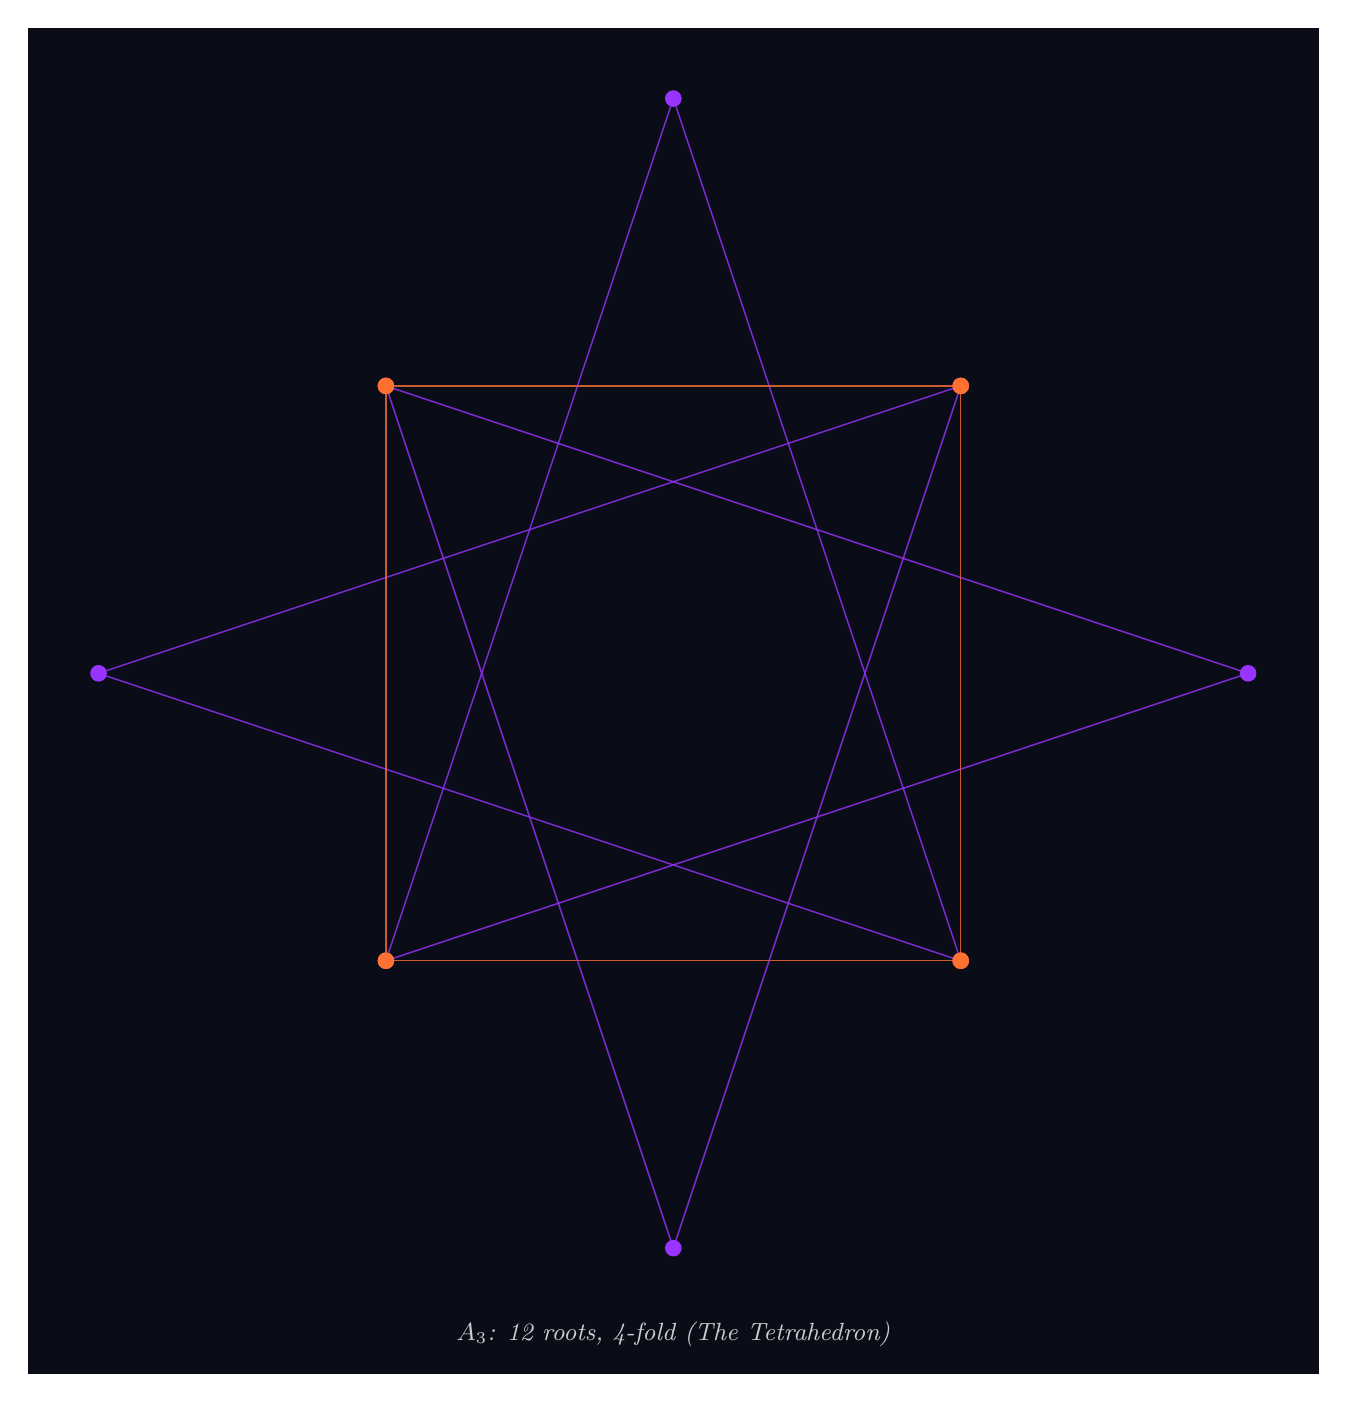
\begin{tikzpicture}
\definecolor{ring0}{rgb}{1.000,0.440,0.200}
\definecolor{ring1}{rgb}{0.600,0.200,1.000}
\definecolor{bg}{rgb}{0.04,0.05,0.09}
\fill[bg] (-8.2,-8.9) rectangle (8.2,8.2);
\draw[ring0,line width=0.5pt,opacity=0.55] (3.650,3.650)--(3.650,-3.650);
\draw[ring1,line width=0.5pt,opacity=0.55] (3.650,3.650)--(-0.000,-7.300);
\draw[ring1,line width=0.5pt,opacity=0.55] (3.650,3.650)--(-7.300,0.000);
\draw[ring0,line width=0.5pt,opacity=0.55] (3.650,3.650)--(-3.650,3.650);
\draw[ring1,line width=0.5pt,opacity=0.55] (7.300,-0.000)--(-3.650,-3.650);
\draw[ring1,line width=0.5pt,opacity=0.55] (7.300,-0.000)--(-3.650,3.650);
\draw[ring1,line width=0.5pt,opacity=0.55] (7.300,-0.000)--(-3.650,-3.650);
\draw[ring1,line width=0.5pt,opacity=0.55] (7.300,-0.000)--(-3.650,3.650);
\draw[ring0,line width=0.5pt,opacity=0.55] (3.650,-3.650)--(-3.650,-3.650);
\draw[ring1,line width=0.5pt,opacity=0.55] (3.650,-3.650)--(-7.300,0.000);
\draw[ring1,line width=0.5pt,opacity=0.55] (3.650,-3.650)--(0.000,7.300);
\draw[ring0,line width=0.5pt,opacity=0.55] (3.650,-3.650)--(3.650,3.650);
\draw[ring0,line width=0.5pt,opacity=0.55] (-3.650,-3.650)--(-3.650,3.650);
\draw[ring1,line width=0.5pt,opacity=0.55] (-3.650,-3.650)--(0.000,7.300);
\draw[ring1,line width=0.5pt,opacity=0.55] (3.650,-3.650)--(-7.300,0.000);
\draw[ring0,line width=0.5pt,opacity=0.55] (3.650,-3.650)--(-3.650,-3.650);
\draw[ring1,line width=0.5pt,opacity=0.55] (3.650,-3.650)--(0.000,7.300);
\draw[ring1,line width=0.5pt,opacity=0.55] (-0.000,-7.300)--(-3.650,3.650);
\draw[ring1,line width=0.5pt,opacity=0.55] (-0.000,-7.300)--(-3.650,3.650);
\draw[ring1,line width=0.5pt,opacity=0.55] (-0.000,-7.300)--(3.650,3.650);
\draw[ring1,line width=0.5pt,opacity=0.55] (-7.300,0.000)--(3.650,3.650);
\draw[ring0,line width=0.5pt,opacity=0.55] (-3.650,3.650)--(3.650,3.650);
\draw[ring0,line width=0.5pt,opacity=0.55] (-3.650,-3.650)--(-3.650,3.650);
\draw[ring1,line width=0.5pt,opacity=0.55] (-3.650,-3.650)--(0.000,7.300);
\fill[ring0] (3.650,3.650) circle (3.0pt);
\fill[ring1] (7.300,-0.000) circle (3.0pt);
\fill[ring0] (3.650,-3.650) circle (3.0pt);
\fill[ring0] (-3.650,-3.650) circle (3.0pt);
\fill[ring0] (3.650,-3.650) circle (3.0pt);
\fill[ring1] (-0.000,-7.300) circle (3.0pt);
\fill[ring1] (-7.300,0.000) circle (3.0pt);
\fill[ring0] (-3.650,3.650) circle (3.0pt);
\fill[ring0] (-3.650,-3.650) circle (3.0pt);
\fill[ring0] (-3.650,3.650) circle (3.0pt);
\fill[ring1] (0.000,7.300) circle (3.0pt);
\fill[ring0] (3.650,3.650) circle (3.0pt);
\node[white!80!black,font=\small\itshape] at (0,-8.4) {$A_3$: 12 roots, 4-fold (The Tetrahedron)};
\end{tikzpicture}
\end{document}